% !Mode:: "TeX:UTF-8"

\documentclass{mcmthesis}
\mcmsetup{CTeX = false,   % 使用 CTeX 套装时,设置为 true
	tcn = {\color{red}67859}, problem = {\color{red}D}
	%        }
	,
	sheet = false, titleinsheet = true, keywordsinsheet = true,
	titlepage = true, abstract = true}
\usepackage{palatino}
\usepackage{enumitem} % Required for manipulating the whitespace between and within lists
\usepackage{listings}
\usepackage{multirow}
\usepackage{nicefrac}
\usepackage{sectsty}
\sectionfont{\color{MidnightBlue}\selectfont}
\subsectionfont{\color{MidnightBlue!50!RoyalBlue}\selectfont}
\subsubsectionfont{\color{SkyBlue!5!RoyalBlue}\selectfont}
\usepackage{booktabs}
\usepackage{lipsum}
\usepackage{varioref} % More descriptive referencing
\setlength\parindent{0pt}
\usepackage{subfig}
%\usepackage[UTF8,nocap]{ctex}
%\usepackage[subfigure,titles]{tocloft}
\usepackage[subfigure]{tocloft}
%\renewcommand\cftsecfont{\color{MidnightBlue}}
%\renewcommand\cftpartpagefont{\color{RoyalBlue}}
%\setlength\cftbeforesecskip{-4pt}
%\setlength\cftbeforesubsecskip{-3.3pt}
%\setlength\cftbeforesubsubsecskip{-5.2pt}
%\renewcommand\cftsecafterpnum{\vskip-4pt}
%\renewcommand{\cftsubsecafterpnum}{\vskip-3.3pt}
%\renewcommand{\cftsubsubsecafterpnum}{\vskip-5.2pt}
%\usepackage[round]{natbib}
%\bibliographystyle{plainnat}
\usepackage{mmstyles}
\usepackage{longtable}
\usepackage{pdflscape}
\usepackage{graphicx}


%\usepackage{subfig} % Required for creating figures with multiple parts (subfigures)
%\usepackage{subfigure}
%\usepackage[square,sort,comma,numbers]{natbib}


\title{Solve   TSP by ILP}
\author{{\itshape Xinglu Wang} \quad {\itshape 3140102282} \quad {\itshape ISEE 1403, ZJU}}
\begin{document}

\maketitle
 
\setcounter{tocdepth}{2} % Set the depth of the table of contents to show sections and subsections only
\tableofcontents
		
\section*{Abstract }
In this report, I  formulate Traveling Salesman Problem (TSP) as  Integer Linear Program (ILP), then collect data for landmarks around HangZhou, use SageMath to solve the ILP and get the exact solution. Although limiting the number of landmarks to $20$, I make some simple comparison with Heuristic Algorithm and visualize the routes on GMap. I find all the procedure  quite interesting and exciting and learn  a lot!

\textbf{Keywords:} TSP, ILP
\section{TSP Problem}
TSP is a combinatorial optimization problem to find the shortest possible Hamiltonian circuit for a complete weighted graph. % \vref{tab:ok}
\subsection{Notation}	 
\begin{table} 
	\centering
	{\begin{tabular}{c|l} 
	\hline
	$\vs = (s_i)$ & At $i$ step, the index of visited city is $s_i$, $ 0 \le i \le n-1$\\
	$\vt= (t_i)$ & City $i$ is visited at step $t_i$, $ 0 \le i \le n-1$\\ \hline \hline
	$\mX = (x_{i j} )$ & Decision variable, $x_{ij}={\begin{cases}1&{\text{the path goes from city }}i{\text{ to city }}j\\0&{\text{otherwise}}\end{cases}}$  \\
	$\pi(\cdot )$ & $\pi(i)=j  \text{ if } x_{i j}=1$, $ 0 \le i,j \le n-1$ \\ \hline \hline
	$\mC=(c_{ij})$ & Cost Matrix \\ 
	\hline
	\end{tabular}
	\caption{The notations that will be used}
	\label{tab:ok}}
\end{table}

There are several key elements:
\begin{itemize}
	\item Hamiltonian circuit means the travel route starting from vertex No. 0, ending at No. 0 and visiting all vertexes once and only once. Note that $x_{ij}|_{i=n-1,j=0}$ denote the distance  go back from No.n-1 to No.0 while  $t_i$ will not consider the time consumed when going back since there is \textit{no} $t_i|_{i=n}$.
	\item It is common for weights of the graph to become non-negative. But for a real-world problem, the weights do no necessarily be symmetric, because weights can represent time or cost. I choose \textit{unsymmetrical}  TSP to solve for its generality ans simplicity Thus, I should be careful that $\mC$ is symmetric because the data I collect is distance while the solution $\mX$ is unsymmetrical because it describe \textit{directed} graph.
\end{itemize} 

\subsection{Formulation as ILP }
We formulate this question step by step, first consider a relaxed version ILP of TSP with some necessary(but not sufficient) constrains:

\begin{align}
\mathop{\mathrm{Minmize \ \  }}       & \sum _{i=0}^{n-1}\sum _{j=0,{\color{Red} j\neq i}}^{n-1}c_{ij}x_{ij} &  & \label{eq:obj}          \\
\mathop{\mathrm{subject \  to \ \  }} & \sum _{i=0,i\neq j}^{n-1}x_{ij}=1                          &  & j=0,\ldots ,n-1;   \label{eq:row}       \\
& \sum _{j=0,j\neq i}^{n-1}x_{ij}=1                          &  & i=0,\ldots ,n-1;         \label{eq:col} \\
& x_{ij} \geq 0, x_{ij} \in \Zbb                                           &  & i,j=0,\ldots ,n-1. \notag
\end{align}

It objective function \eqref{eq:obj} (and all the following  equations  throughout the problem), we simply drop $x_{ii}$, since $x_{ii}=0$ is trivial. The constrain \eqref{eq:row} means each city be arrived at from exactly one other city while equation \eqref{eq:col} means from each city there is a departure to exactly one other city. We do not need to add $x_{ij} \le 1 $ since the rests are enough to conclude it. 

But these constraints are not sufficient conditions for TSP. This formulation is, in fact, the ILP formulation of Assignment Problem which belong to P hard class. We still need to add constraints to avoid subtour and we will find that TSP belong to NP hard   class. Next we will add $n$ auxiliary variables so that we just need to add $n(n-1)$ constrain. 
\begin{align}
	\mathop{\mathrm{Minmize \ \  }}       & \sum _{i=0}^{n-1}\sum _{j=0,j\neq i}^{n-1}c_{ij}x_{ij} &  & \notag                     \\
	\mathop{\mathrm{subject \  to \ \  }} & \sum _{i=0,i\neq j}^{n-1}x_{ij}=1                    &  & j=0,\ldots ,n-1;  \notag     \\
	                                      & \sum _{j=0,j\neq i}^{n-1}x_{ij}=1                    &  & i=0,\ldots ,n-1;      \notag \\
	                                      & \color{Blue} t_{j} \ge t_{i}+1-n(1-x_{ij})x  &  & 0\leq i\leq n-1, {\color{Red}1 \le} j \le n-1, i \neq j   \label{eq:new}     \\
	                                      & x_{ij} \geq 0, x_{ij} \in \Zbb                     &  & i,j=0,\ldots ,n-1. \notag
\end{align}
Note that $j \ge 1 $ in \eqref{eq:new} means we do not consider salesman going back to No.0. In fact, if we let $t_{n}$ denote the time step salesman go back to No.0, we have:
\begin{equation}\label{eq:my}
t_{n}=t_{n-1}+1=n 
\end{equation}
 Then we prove that this ILP is equivalent to TSP. \quad \textbf{(I).} cyclic permutation without subtour conclude constraint \eqref{eq:new}. Because \eqref{eq:new} is equivalent to statement that   if the next visited city for $i$ is $j$ ($x_{ij}=1$) ,then $t_j=t_i+1$. If $x_{ij}=0$, then we add a trivial constraint $t_j \ge t_j +1-n$.  The equivalent statement is satisfied.  \quad \textbf{(II).} constraint \eqref{eq:new} eliminates all subtour. We can prove it by tricky reductio ad absurdum. Suppose the feasible solution $\mX$ contain more than one subtour. Then there exist $\vs=(i_1,\dots,i_r)$ not containing 0. Note that $i_r$ in this circle will go back to $i_1$, so there is additional equation $t_{i_1}=t_{i_r}+1$  quite different with \eqref{eq:my}. Go along this cycle, we find that $0=r$, and the contradiction lies in the fact that the cycle do not containing 0.

\section{Experiments}

The steps to solve the ILP include: 
\begin{itemize}[noitemsep,nolistsep]
	\item Collect location data for landmarks around HangZhou. 
	\item Transform from (latitude,longitude)  to distance matrix $\mC$. Following guide of \href{https://en.wikipedia.org/wiki/Haversine_formula}{Haversine\_formula}. 
	\item Solve the ILP by MILP class. The equivalent code for ILP system \eqref{eq:new} is more human-friendly and powerful compared with \textit{`intlinprog`} function of Matlab.  Ref. to \vref{code:sage}. I put the code in the Appendix, hope do not impact the compactness of this report.
	\item Visualize on GMap. 
\end{itemize}
%\begin{lstlisting}[language=Python]
%p=MixedIntegerLinearProgram(maximization=False) 
%# Define Varibles:
%x=p.new_variable(nonnegative=True,integer=True)
%t=p.new_variable(nonnegative=True,integer=True)
%n=dist.nrows()
%obj_func=0
%# Define Obj Function:
%for i in range(n):
%	for j in range(n):
%		obj_func+=x[i,j]*dist[i,j] if i!=j else 0
%p.set_objective(obj_func)
%# Add Constrains
%for i in range(n):
%	p.add_constraint(sum([x[i,j] for j in range(n) if i!=j ])==1)
%for j in range(n):
%	p.add_constraint(sum([x[i,j] for i in range(n) if i!=j ])==1)
%for i in range(n):
%	for j in range(1,n):
%		if i==j :
%			continue
%		p.add_constraint(t[j]>=t[i]+1-n*(1-x[i,j]))
%for i in range(n):
%	p.add_constraint(t[i]<=n-1)
%
%#p.show()
%p.solve()
%\end{lstlisting}

Apply ILP to a toy case with 20 landmarks around HangZhou, we get a optimal strategy to travel around HangZhou. It is quite interesting and exciting. Ref. to Fig~\vref{fig:tsp_res}. Then I also use TSP solver in Sage to partially verify that my code is correct. The approximate optimal solution got by some heuristic algorithm is the same as the exact optimal solution. I make some try, and guess that when $n$ is small, it is easier for heuristic algorithm to find exact optimal solution.  Then I also try to travel around JiangZheHu Region(Yangtze River delta) and visualize it on the map, Ref. to Fig~\vref{fig:jiangzhehu}. 

\begin{figure}
	\centering
	\subfloat[Initial feasible solution for TSP]{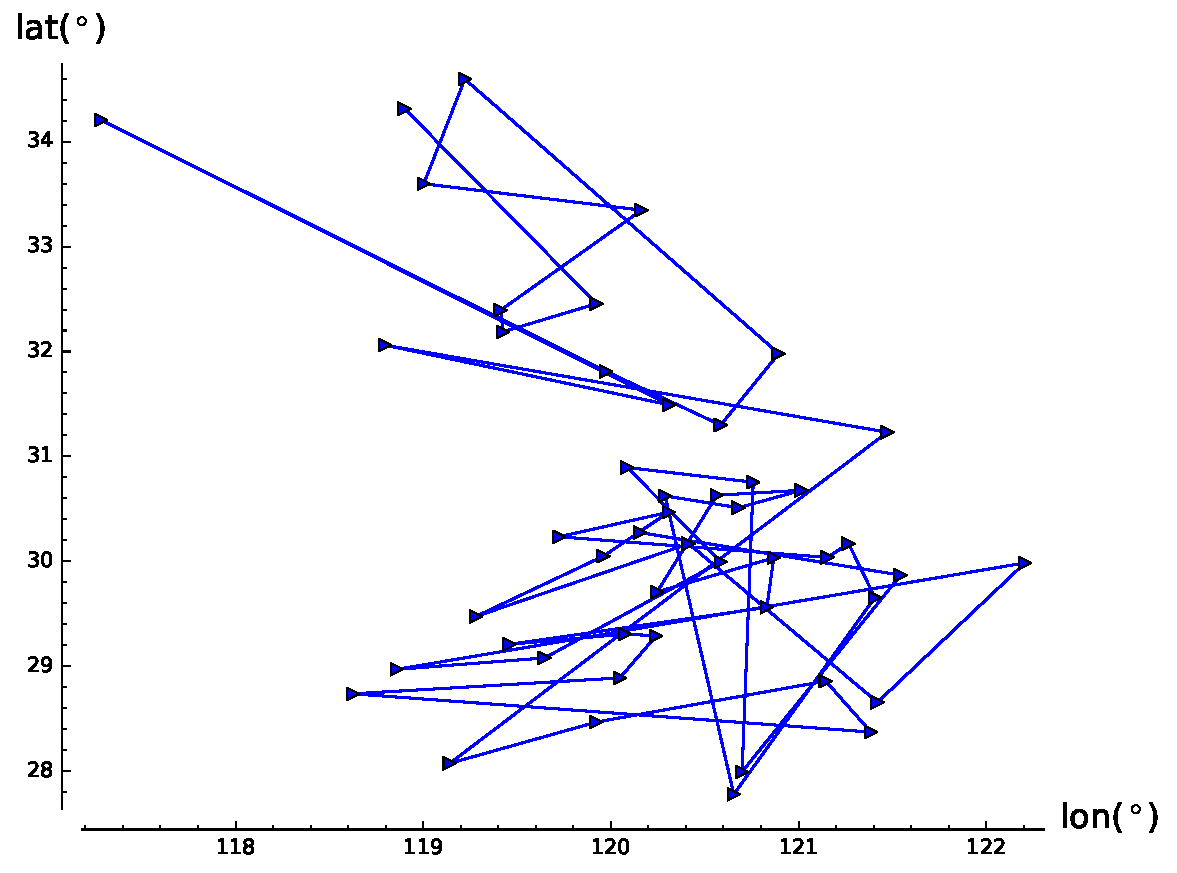
\includegraphics[width=.3\columnwidth]{init_map}} \quad  
	\subfloat[Transform into complete weight graph]{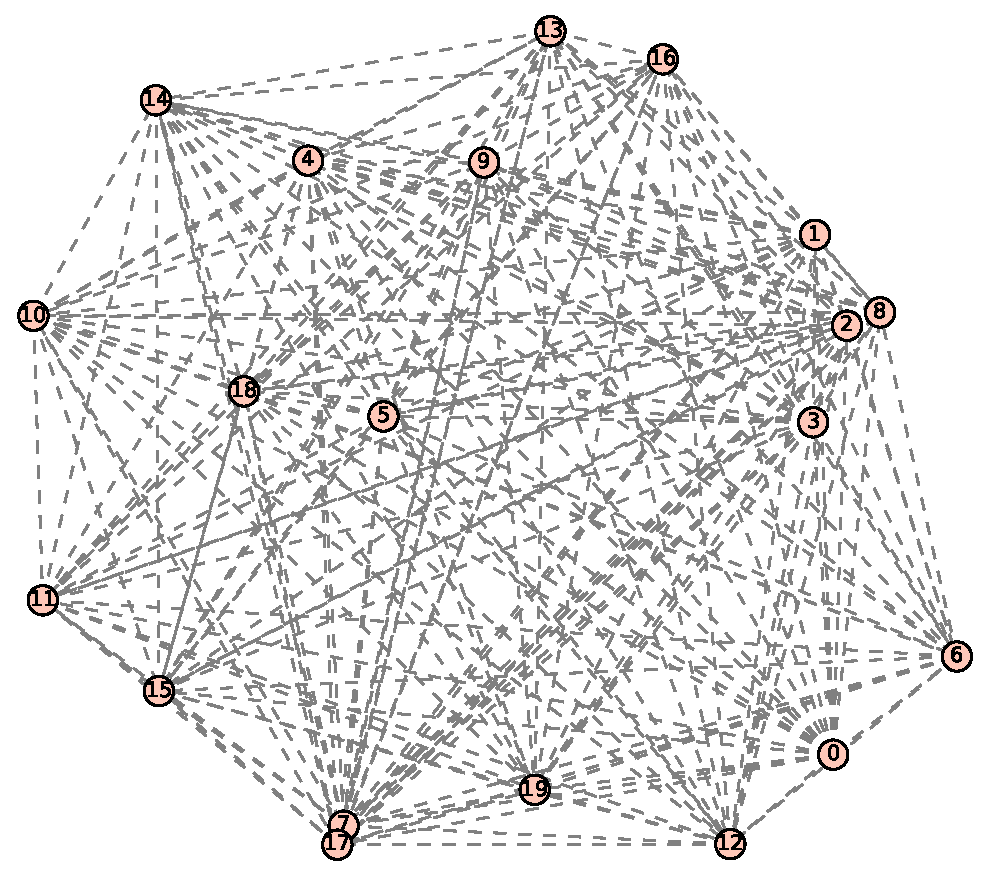
\includegraphics[width=.25\columnwidth]{topology}}  \quad
	\subfloat[Plot according to locations]{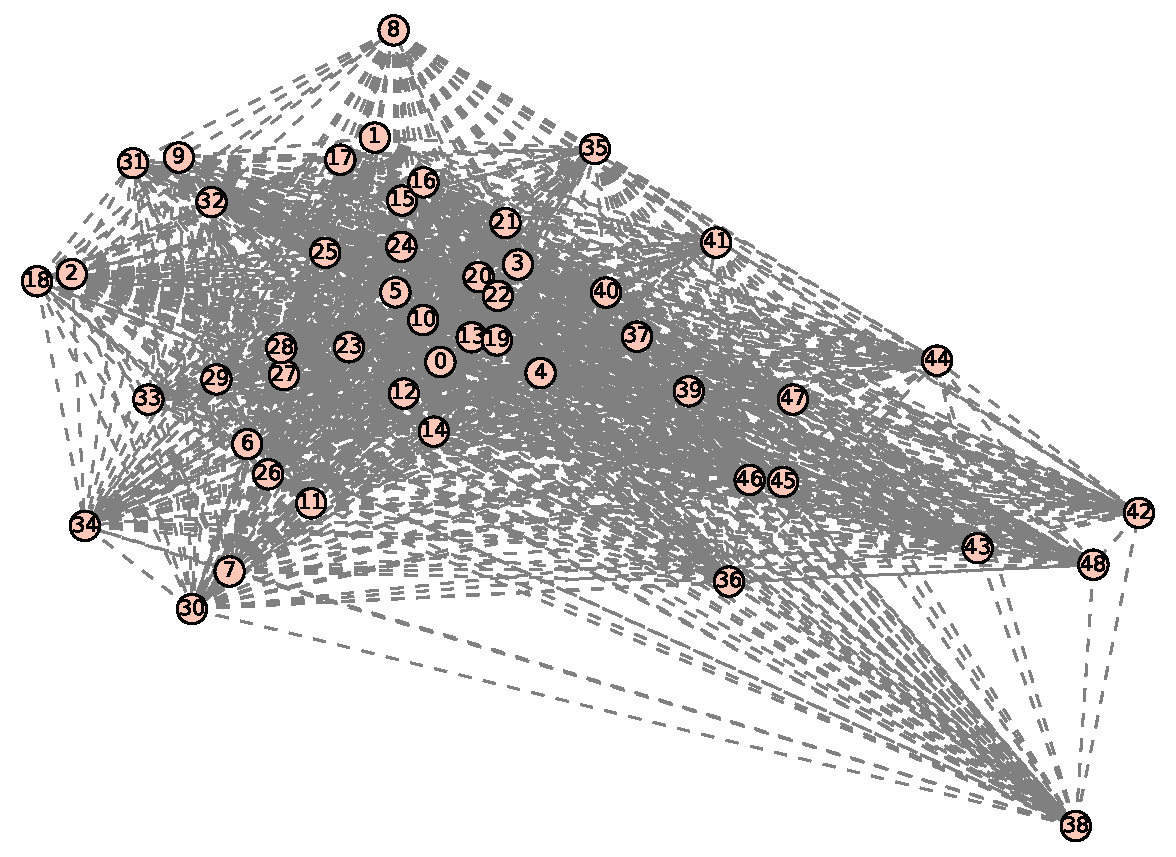
\includegraphics[width=.35\columnwidth]{trans_map}}
	\\
	\subfloat[The optimal solution find by ILP]{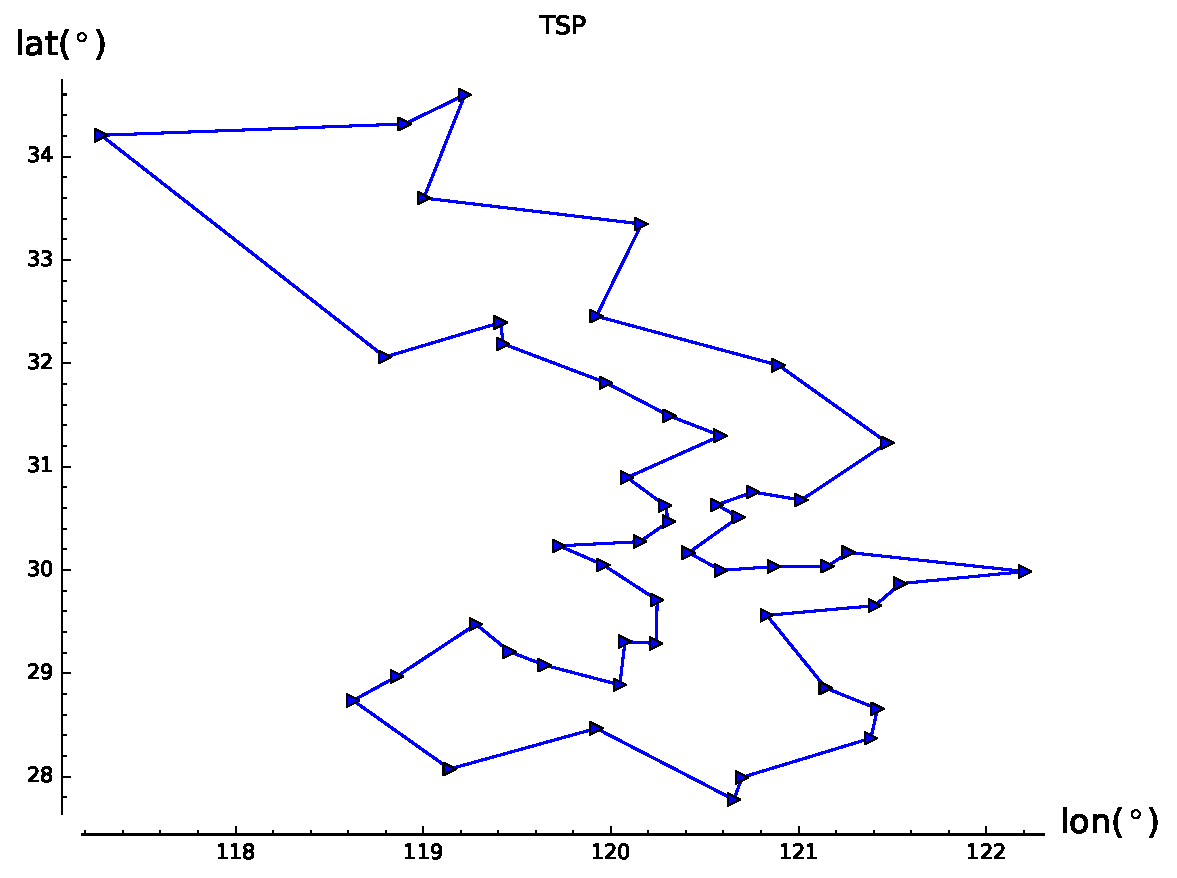
\includegraphics[width=.4\columnwidth]{tsp_res}\label{fig:tsp_res}}  \quad 
	\subfloat[Approximately optimal find by Sage]{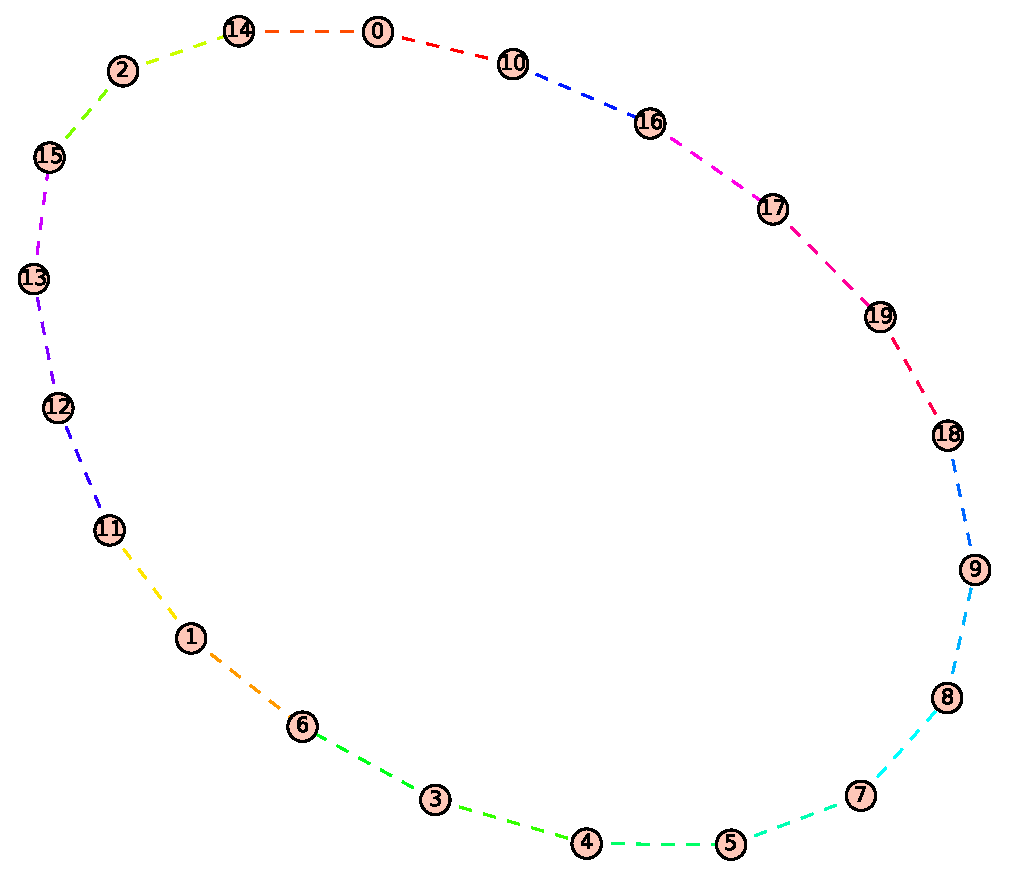
\includegraphics[width=.4\columnwidth]{tsp_sage} \label{fig:tsp_sage} }
	\caption[Results]{The plot  of  TSP class \vref{fig:tsp_sage} only keep topological relations, but after simple transformation, we find for 20-pts, two solutions $\mX$ are equivalent. (Here the transformation means change from undirected graph's $\mX=(x_{ij})$ with $i < j$  to directed graph's $\mX$ ) } 
\end{figure}
\begin{figure}
	\centering
	\subfloat[TSP on Hangzhou]{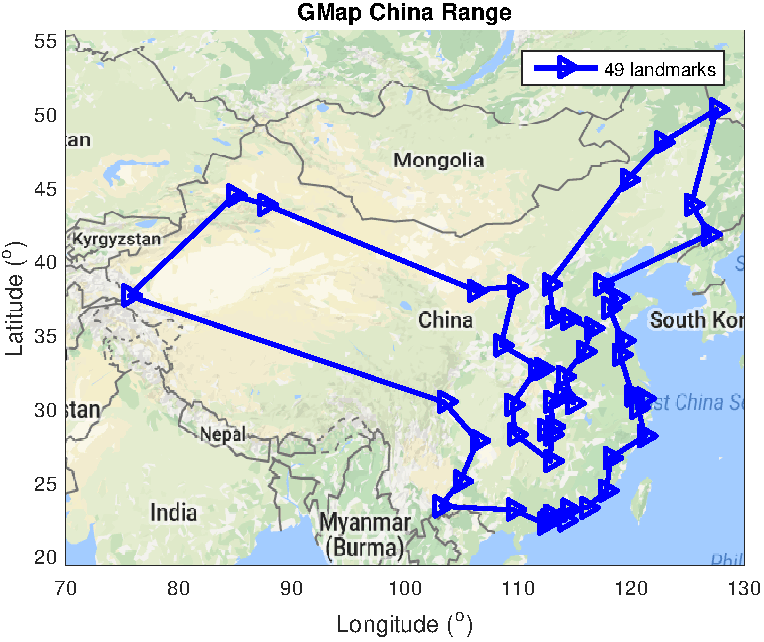
\includegraphics[width=.48\columnwidth]{GMap_Cn}} \   
	\subfloat[TSP on JiangZheHu]{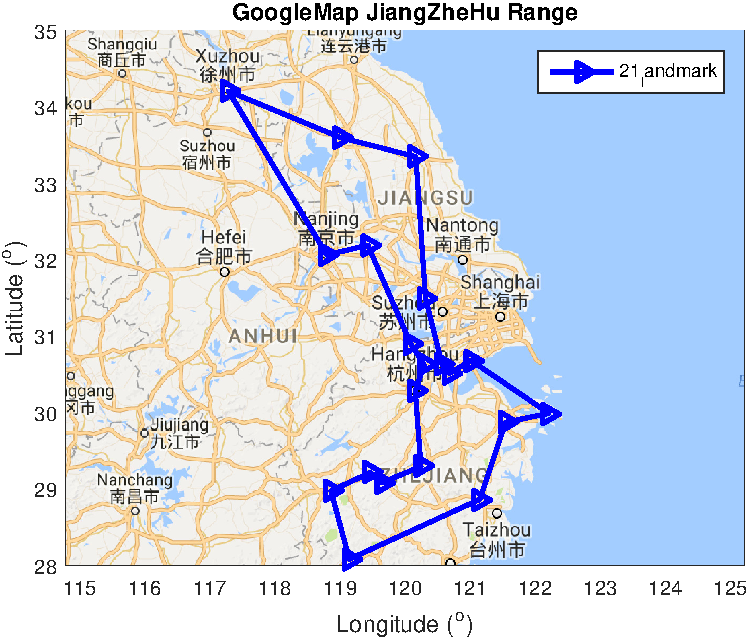
\includegraphics[width=.47\columnwidth]{GMap_Jzh}\label{fig:jiangzhehu}} 
	\caption[Results]{JiangZheHu is a wider range than Hangzhou. We limit number of landmarks to about 20 for speed.} 
\end{figure}

I just take 20 landmarks from 49 collected coordinate data. The reason lies in  the fact that I find 50 points consume seemingly endless time. I also have some basic test on running time, and find it grow explosively(and unstably), Ref. to Fig~\vref{fig:elaspe}. We can conclude that the time complexity of  branch-bound method is of  exponential time complexity.

\begin{figure}[h]
	\centering
	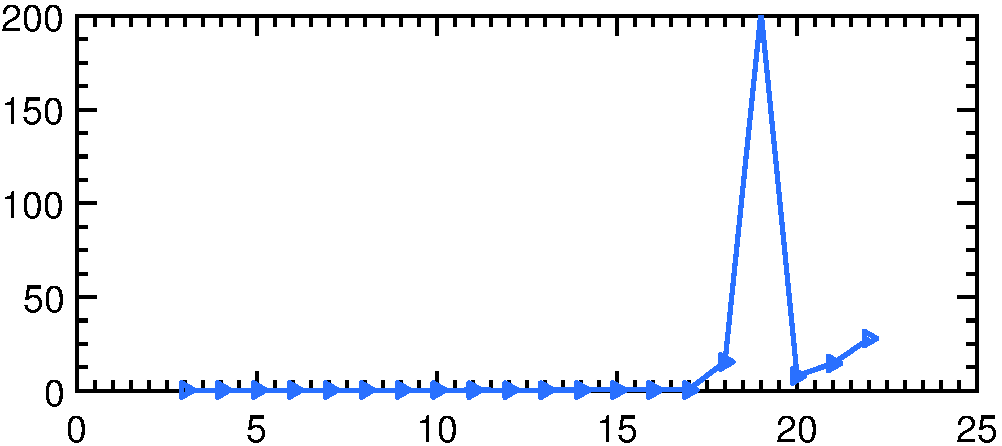
\includegraphics[width=.5\columnwidth]{benchmark}
	\caption[Running time]{X-axis: number of landmarks, Y-axis: elapsed time in seconds. Running time starts to grow explosively at $n=17$ and becomes $200s$  at  $n=19$  suddenly.}
	\label{fig:elaspe}.
\end{figure}
		

\begin{appendices}
\section{Lab Code}
My codes are somewhat lengthy, so I just put some important code, hope not to impact the compactness of this report. 
	\subsection{Crawling Data of CHINA Landmarks}
	\lstinputlisting[language=Python]{./code/test.py}
	\subsection{Solve by Sage} \label{code:sage}
	\lstinputlisting[language=Python]{./code/sage.py}
	\lstinputlisting[language=Python]{./code/sage2.py}
	\subsection{Draw on GMap}
	\lstinputlisting[language=Matlab]{./code/lOptHw.m}	
	%\textbf{\textcolor[rgb]{0.98,0.00,0.00}{Input matlab source:}}
	
	%some more text \textcolor[rgb]{0.98,0.00,0.00}{\textbf{Input C++ source:}}
	%\lstinputlisting[language=C++]{./code/mcmthesis-sudoku.cpp}
	
%			\section{Landmarks Around HangZhou }
%			\begin{longtable}{|l||l|l|} \hline
city & latitude & longitude \\ \hline \hline
$\text{\texttt{Hangzhou}}$ & $30.274085$ & $120.15507$ \\ \hline
$\text{\texttt{Ningbo}}$ & $29.868336$ & $121.54399$ \\ \hline
$\text{\texttt{Wenzhou}}$ & $27.993828$ & $120.699362$ \\ \hline
$\text{\texttt{Jiaxing}}$ & $30.753924$ & $120.758543$ \\ \hline
$\text{\texttt{Huzhou}}$ & $30.894348$ & $120.086823$ \\ \hline
$\text{\texttt{Shaoxing}}$ & $29.995762$ & $120.586109$ \\ \hline
$\text{\texttt{Jinhua}}$ & $29.079175$ & $119.647421$ \\ \hline
$\text{\texttt{Quzhou}}$ & $28.97008$ & $118.859457$ \\ \hline
$\text{\texttt{Zhoushan}}$ & $29.985295$ & $122.207216$ \\ \hline
$\text{\texttt{Taizhou}}$ & $28.65638$ & $121.42076$ \\ \hline
$\text{\texttt{Xiaoshan}}$ & $30.168016$ & $120.414929$ \\ \hline
$\text{\texttt{Jiande}}$ & $29.474871$ & $119.281164$ \\ \hline
$\text{\texttt{Fuyang}}$ & $30.048692$ & $119.960076$ \\ \hline
$\text{\texttt{Yongning{ }Rd}}$ & $30.4682595$ & $120.308662$ \\ \hline
$\text{\texttt{Lin'an}}$ & $30.233873$ & $119.724733$ \\ \hline
$\text{\texttt{Yuyao}}$ & $30.037192$ & $121.154634$ \\ \hline
$\text{\texttt{Cixi}}$ & $30.169665$ & $121.266579$ \\ \hline
$\text{\texttt{Fenghua}}$ & $29.655143$ & $121.406995$ \\ \hline
$\text{\texttt{Rui'an}}$ & $27.778657$ & $120.655148$ \\ \hline
$\text{\texttt{Deqing}}$ & $30.623883$ & $120.289015$ \\ \hline
$\text{\texttt{Haining}}$ & $30.510659$ & $120.680757$ \\ \hline
$\text{\texttt{Pinghu}}$ & $30.677233$ & $121.015142$ \\ \hline
$\text{\texttt{Tongxiang}}$ & $30.630173$ & $120.565099$ \\ \hline
$\text{\texttt{Zhuji}}$ & $29.708692$ & $120.246863$ \\ \hline
$\text{\texttt{Shangyu}}$ & $30.033121$ & $120.868122$ \\ \hline
$\text{\texttt{Shengzhou}}$ & $29.56141$ & $120.831026$ \\ \hline
$\text{\texttt{Lanxi}}$ & $29.208919$ & $119.460526$ \\ \hline
$\text{\texttt{Yiwu}}$ & $29.306757$ & $120.07514$ \\ \hline
$\text{\texttt{Dongyang}}$ & $29.289648$ & $120.241566$ \\ \hline
$\text{\texttt{Yongkang}}$ & $28.888555$ & $120.047651$ \\ \hline
$\text{\texttt{Jiangshan}}$ & $28.737223$ & $118.626974$ \\ \hline
$\text{\texttt{Wenling}}$ & $28.372506$ & $121.385604$ \\ \hline
$\text{\texttt{Linhai}}$ & $28.858457$ & $121.145046$ \\ \hline
$\text{\texttt{Lishui}}$ & $28.46763$ & $119.922796$ \\ \hline
$\text{\texttt{Longquan}}$ & $28.07465$ & $119.141474$ \\ \hline
$\text{\texttt{Shanghai}}$ & $31.230416$ & $121.473701$ \\ \hline
$\text{\texttt{Nanjing}}$ & $32.060255$ & $118.796877$ \\ \hline
$\text{\texttt{Wuxi}}$ & $31.49117$ & $120.31191$ \\ \hline
$\text{\texttt{Xuzhou}}$ & $34.205768$ & $117.284124$ \\ \hline
$\text{\texttt{Changzhou}}$ & $31.811226$ & $119.974062$ \\ \hline
$\text{\texttt{Suzhou}}$ & $31.298979$ & $120.58529$ \\ \hline
$\text{\texttt{Nantong}}$ & $31.980172$ & $120.894291$ \\ \hline
$\text{\texttt{Lianyungang}}$ & $34.596653$ & $119.221611$ \\ \hline
$\text{\texttt{9{ }Xueyuan{ }Rd}}$ & $33.598607$ & $119.0033924$ \\ \hline
$\text{\texttt{Yancheng}}$ & $33.347316$ & $120.16366$ \\ \hline
$\text{\texttt{Yangzhou}}$ & $32.394213$ & $119.412947$ \\ \hline
$\text{\texttt{Zhenjiang}}$ & $32.187849$ & $119.425836$ \\ \hline
$\text{\texttt{Taizhou}}$ & $32.455536$ & $119.922933$ \\ \hline
$\text{\texttt{745{ }Country{ }Rd}}$ & $34.3147372$ & $118.901079$ \\ \hline
\end{longtable}		
\end{appendices}

\begin{thebibliography}{99}
	\bibitem{bib:o} \url{http://www.openstreetmap.org/export#map=16/30.2802/120.1700}
	\bibitem{bib:github/sage/tsp} \url{https://github.com/sagemath/sagelib/blob/master/sage/graphs/generic_graph.py}	
	
\end{thebibliography}
	
\end{document}